% SC4053 --- Chapter 4: Smart Contracts (Solidity/EVM) (0->100)
\chapter{Smart Contracts: Solidity and the EVM}\label{ch:contracts}

\begin{quote}
\emph{``A smart contract is a program that lives on the chain, holds money, and runs exactly as written -- whether the author regrets it afterwards or not.''} --- We learn to write, trace and defend such programs.
\end{quote}

\noindent\fbox{\parbox{\dimexpr\linewidth-2\fboxsep-2\fboxrule}{%
\textbf{From zero: no EVM background assumed.} We start from a vending machine (insert coin, get soda, no clerk) and turn it into code that lives on the blockchain. We define gas, storage, calldata and ABI from first principles before writing a line of Solidity.}}
\vspace{0.4em}

\section*{Learning Outcomes}
After this chapter you will be able to:
\begin{enumerate}[label=(L\arabic*)]
    \item write, compile and deploy a Solidity contract and call it via its ABI;
    \item trace EVM execution: stack, memory, storage, calldata and gas accounting;
    \item explain events, logs and the difference between \texttt{call} and \texttt{delegatecall};
    \item identify and fix reentrancy, integer and access-control bugs;
    \item test with Hardhat/Foundry and estimate gas.
\end{enumerate}

% ============================================================
\section{From Vending Machines to On-Chain Programs}\label{sec:vending}
A \emph{smart contract} is deterministic code stored at an address. Anyone can send a transaction to that address with input data; every honest node re-executes the code and agrees on the outcome. The contract can hold ether/tokens, update persistent storage, and call other contracts. The key difference from a server: execution is \emph{replicated and metered} -- every node runs it, and every operation costs gas so infinite loops cannot halt the chain.

Two properties dominate design:
\begin{description}[leftmargin=1.2em,style=nextline]
    \item[Determinism] No randomness, wall-clock or network I/O -- all nodes must reach the same result from the same state and input.
    \item[Gas metering] Each EVM opcode has a gas price (e.g., \texttt{ADD}=3, \texttt{SSTORE}=20000). The transaction specifies a gas limit; exceeding it reverts.
\end{description}

% ============================================================
\section{The EVM Execution Model}\label{sec:evm}
The EVM is a stack machine with three data areas:

\begin{figure}[h]\centering
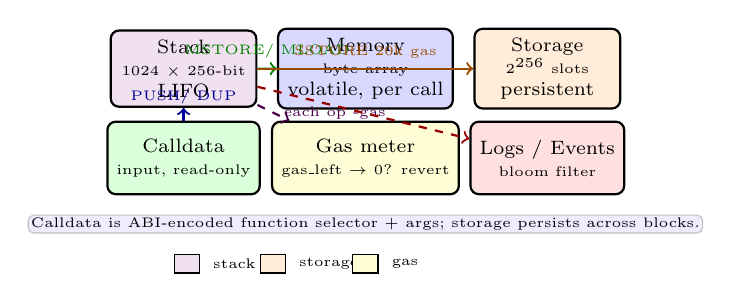
\begin{tikzpicture}[scale=0.84, every node/.style={font=\scriptsize},
  box/.style={draw,rounded corners=3pt,minimum width=1.85cm,minimum height=0.92cm,align=center,thick}]
\node[box,fill=violet!12] (stk) at (0,1.80) {Stack\\ \tiny 1024 $\times$ 256-bit\\ LIFO};
\node[box,fill=blue!15] (mem) at (2.75,1.80) {Memory\\ \tiny byte array\\ volatile, per call};
\node[box,fill=orange!15] (sto) at (5.50,1.80) {Storage\\ \tiny $2^{256}$ slots\\ persistent};
\node[box,fill=green!14] (cal) at (0,0.45) {Calldata\\ \tiny input, read-only};
\node[box,fill=yellow!16] (gas) at (2.75,0.45) {Gas meter\\ \tiny gas\_left $\to$ 0? revert};
\node[box,fill=red!12] (log) at (5.50,0.45) {Logs / Events\\ \tiny bloom filter};
\draw[->,thick,blue!60!black] (cal)--(stk) node[midway,above,font=\tiny] {PUSH/ DUP};
\draw[->,thick,green!50!black] (stk)--(mem) node[midway,above,font=\tiny] {MSTORE/ MLOAD};
\draw[->,thick,orange!60!black] (stk)--(sto) node[midway,above,font=\tiny] {SSTORE 20k gas};
\draw[->,thick,violet!60!black,dashed] (stk)--(gas) node[midway,right,font=\tiny] {each op -gas};
\draw[->,thick,red!60!black,dashed] (stk)--(log);
\node[font=\tiny,fill=blue!7,draw=gray!50,rounded corners=2pt,inner sep=1pt,align=center] at (2.75,-0.55) {Calldata is ABI-encoded function selector + args; storage persists across blocks.};
% legend
\node[draw,fill=violet!12,minimum width=0.32cm,minimum height=0.18cm] at (0.05,-1.15) {}; \node[font=\tiny,anchor=west] at (0.30,-1.15) {stack};
\node[draw,fill=orange!15,minimum width=0.32cm,minimum height=0.18cm] at (1.35,-1.15) {}; \node[font=\tiny,anchor=west] at (1.60,-1.15) {storage};
\node[draw,fill=yellow!16,minimum width=0.32cm,minimum height=0.18cm] at (2.75,-1.15) {}; \node[font=\tiny,anchor=west] at (3.00,-1.15) {gas};
\end{tikzpicture}
\caption{EVM machine model: a stack drives computation, memory is scratch space, storage is the durable key-value map, calldata carries the ABI-encoded call, and the gas meter halts runaway execution. Colour distinguishes volatile vs persistent areas.}
\label{fig:evm-model}
\end{figure}

\begin{example}[ABI encoding]\label{ex:abi}
Calling \texttt{transfer(address,uint256)} with args \texttt{(0xABC...,100)} encodes as 4-byte selector \texttt{0xa9059cbb} plus two 32-byte padded words. The EVM's calldata is exactly those 68 bytes. Decoding is the callee's first act.
\end{example}

\subsection{Calls and delegatecall}\label{subsec:calls}
\begin{itemize}[leftmargin=1.2em]
    \item \texttt{addr.call(data)} runs callee code with callee storage, \texttt{msg.sender}=caller address.
    \item \texttt{addr.delegatecall(data)} runs callee code \emph{with caller storage} -- powerful for proxies but dangerous if mis-authorised.
\end{itemize}

\begin{figure}[h]\centering
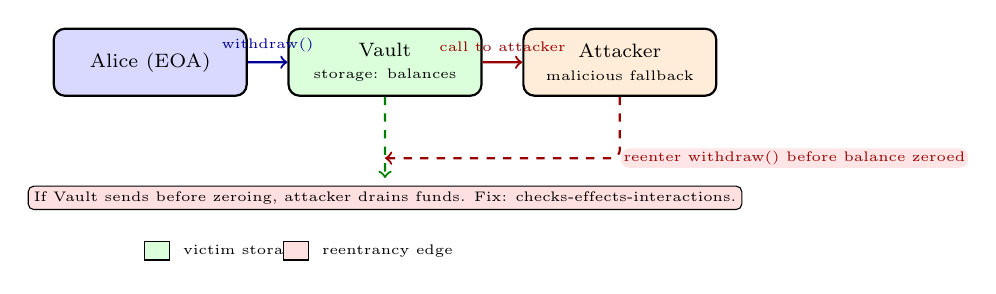
\begin{tikzpicture}[scale=0.84, every node/.style={font=\scriptsize},
  ctr/.style={draw,rounded corners=4pt,minimum width=2.45cm,minimum height=0.85cm,align=center,thick}]
\node[ctr,fill=blue!15] (alice) at (0,2.10) {Alice (EOA)};
\node[ctr,fill=green!14] (vault) at (3.55,2.10) {Vault\\ \tiny storage: balances};
\node[ctr,fill=orange!15] (atk) at (7.10,2.10) {Attacker\\ \tiny malicious fallback};
\draw[->,thick,blue!60!black] (alice)--(vault) node[midway,above,font=\tiny] {withdraw()};
\draw[->,thick,red!60!black] (vault)--(atk) node[midway,above,font=\tiny] {call to attacker};
\draw[->,thick,red!60!black,dashed,rounded corners=3pt] (atk) |- (3.55,0.65) node[midway,right,font=\tiny,fill=red!10,inner sep=1pt] {reenter withdraw() before balance zeroed};
\node[draw,fill=red!12,rounded corners=2pt,inner sep=2pt,font=\tiny,align=center] at (3.55,0.05) {If Vault sends before zeroing, attacker drains funds. Fix: checks-effects-interactions.};
\draw[->,thick,green!50!black,dashed] (vault.south) -- (3.55,0.35);
% legend
\node[draw,fill=green!14,minimum width=0.32cm,minimum height=0.18cm] at (0.10,-0.75) {}; \node[font=\tiny,anchor=west] at (0.35,-0.75) {victim storage};
\node[draw,fill=red!12,minimum width=0.32cm,minimum height=0.18cm] at (2.20,-0.75) {}; \node[font=\tiny,anchor=west] at (2.45,-0.75) {reentrancy edge};
\end{tikzpicture}
\caption{Reentrancy: the vault calls the attacker, which reenters the vault before the first call updates storage. Colour highlights victim vs attacker control.}
\label{fig:reentrancy}
\end{figure}

% ============================================================
\section{Writing Solidity}\label{sec:solidity}

\begin{lstlisting}[language=Solidity]
// SPDX-License-Identifier: MIT
pragma solidity ^0.8.20;

contract SimpleVault {
    mapping(address => uint256) public balances;
    event Deposit(address indexed who, uint256 amount);
    event Withdraw(address indexed who, uint256 amount);

    function deposit() external payable {
        balances[msg.sender] += msg.value;
        emit Deposit(msg.sender, msg.value);
    }
    // VULNERABLE version -- for teaching (do NOT deploy)
    function withdrawVuln() external {
        uint256 bal = balances[msg.sender];
        require(bal > 0, "empty");
        (bool ok, ) = msg.sender.call{value: bal}(""); // external call first
        require(ok, "send fail");
        balances[msg.sender] = 0; // too late -- reentrancy!
    }
    // FIXED: checks-effects-interactions + guard
    bool private locked;
    modifier noReentrancy(){ require(!locked, "locked"); locked=true; _; locked=false; }
    function withdraw() external noReentrancy {
        uint256 bal = balances[msg.sender];
        require(bal > 0, "empty");
        balances[msg.sender] = 0; // effects before interaction
        (bool ok, ) = msg.sender.call{value: bal}("");
        require(ok, "send fail");
        emit Withdraw(msg.sender, bal);
    }
}
\end{lstlisting}

Key patterns: \emph{checks-effects-interactions} (update storage before external calls), \emph{reentrancy guard}, \emph{pull over push}, and \emph{pausable/ownable} for emergencies.

\begin{lstlisting}[language=Python]
# Gas estimator (teaching -- real costs from Yellow Paper Table G)
GAS = {"ADD":3,"MUL":5,"SSTORE_new":20000,"SSTORE_reset":2900,"SLOAD":2100,
       "CALL":700,"MSTORE":3,"KECCAK":30}
def estimate(ops):
    return sum(GAS[o] for o in ops)
print("withdraw trace cost:", estimate(["SLOAD","CALL","SSTORE_reset"]))
# -> 9700 gas sketch; real trace includes memory expansion etc.
# ABI encode helper
import hashlib
def selector(sig): return hashlib.sha3_256(sig.encode()).hexdigest()[:8]
# Note: use keccak (not sha3 NIST) in production; hashlib.sha3 is close for demo
print("transfer selector demo:", selector("transfer(address,uint256)"))
\end{lstlisting}

\subsection{Errors that cost millions}\label{subsec:errors}
Three patterns have drained hundreds of millions: (1) \emph{reentrancy} above; (2) \emph{unchecked call return} -- low-level \texttt{call} returns false on failure instead of reverting, so ignoring the bool silently loses funds; (3) \emph{access control} -- missing \texttt{onlyOwner} lets anyone call \texttt{selfdestruct} or mint. Solidity 0.8's checked arithmetic fixed a fourth class (overflow), but price-oracle manipulation (using a spot AMM price as truth) remains subtle. The fix for each is a small code change, which is why audit checklists are so valuable.

\begin{example}[Unchecked call]\label{ex:unchecked}
\texttt{addr.call\{value:1 ether\}("")} without checking \texttt{ok} can fail (out-of-gas, recipient reverts) while the vault thinks it succeeded and zeroes the balance anyway. Always write \texttt{require(ok)} or use OpenZeppelin's \texttt{Address.sendValue}.
\end{example}

\begin{remark}[Testing philosophy]\label{rem:testing}
Tests should cover \emph{unit} (single function), \emph{integration} (contract-to-contract calls), and \emph{invariant/fuzz} (random sequences must preserve e.g.\ total deposits = contract balance + total withdrawn). Foundry's \texttt{forge test --fuzz} and Halmos symbolic execution automate the last class.
\end{remark}

\begin{figure}[h]\centering
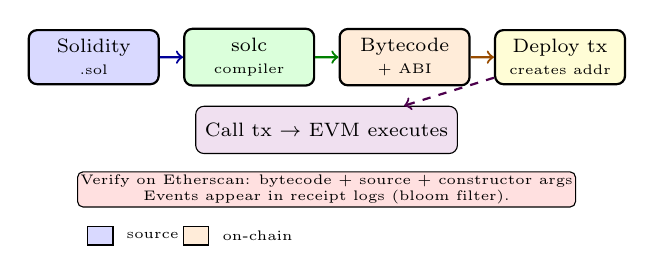
\begin{tikzpicture}[scale=0.84, every node/.style={font=\scriptsize},
  mystep/.style={draw,rounded corners=3pt,minimum width=1.65cm,minimum height=0.60cm,align=center,thick}]
\node[mystep,fill=blue!15] (src) at (0,1.65) {Solidity\\ \tiny .sol};
\node[mystep,fill=green!14] (cmp) at (2.35,1.65) {solc\\ \tiny compiler};
\node[mystep,fill=orange!15] (byte) at (4.70,1.65) {Bytecode\\ \tiny + ABI};
\node[mystep,fill=yellow!16] (dep) at (7.05,1.65) {Deploy tx\\ \tiny creates addr};
\draw[->,thick,blue!60!black] (src)--(cmp); \draw[->,thick,green!50!black] (cmp)--(byte); \draw[->,thick,orange!60!black] (byte)--(dep);
\node[draw,fill=violet!12,rounded corners=3pt,minimum width=2.25cm,minimum height=0.60cm,align=center] (call) at (3.52,0.55) {Call tx $\to$ EVM executes};
\draw[->,thick,violet!60!black,dashed] (dep)--(call);
\node[draw,fill=red!12,rounded corners=2pt,inner sep=1pt,font=\tiny,align=center] at (3.52,-0.35) {Verify on Etherscan: bytecode + source + constructor args\\Events appear in receipt logs (bloom filter).};
% legend
\node[draw,fill=blue!15,minimum width=0.32cm,minimum height=0.18cm] at (0.10,-1.05) {}; \node[font=\tiny,anchor=west] at (0.35,-1.05) {source};
\node[draw,fill=orange!15,minimum width=0.32cm,minimum height=0.18cm] at (1.55,-1.05) {}; \node[font=\tiny,anchor=west] at (1.80,-1.05) {on-chain};
\end{tikzpicture}
\caption{Contract lifecycle: source $\to$ bytecode/ABI $\to$ deploy transaction $\to$ on-chain address. Off-chain tools (Hardhat, Foundry) automate compile, test and verify steps.}
\label{fig:deploy-pipe}
\end{figure}

% ============================================================
\section{Exercises}\label{sec:ch04-exercises}
\begin{enumerate}[label=E4.\arabic*, leftmargin=*, itemsep=0.6em]
    \item \textbf{ABI drill.} Encode \texttt{transfer(0x1234...abcd, 1000)} by hand (selector + two words). Decode a given calldata hex back to function and args.
    \item \textbf{Reentrancy exploit.} Write an attacker contract that reenters \texttt{withdrawVuln} three times. Trace balances and call stack depth at each reentry. Then show why \texttt{withdraw} (fixed) blocks it.
    \item \textbf{Gas golf.} Given a loop that does \texttt{SSTORE} per iteration, estimate total gas for 100 iterations (new vs reset slots). Propose a packing that halves storage writes.
    \item \textbf{delegatecall danger.} A proxy uses \texttt{delegatecall} to a logic contract that has a \texttt{selfdestruct}. Explain how an attacker can destroy the proxy. What is the fix (UUPS vs transparent proxy)?
    \item \textbf{Test harness.} Write a Foundry/Hardhat test that deposits, withdraws and checks events for \texttt{SimpleVault}. Add a fuzz test that tries random deposit/withdraw sequences and asserts conservation.
\end{enumerate}

\begin{remark}[Upgradeability]\label{rem:upgrade}
Because contracts are immutable, teams use \emph{proxy} patterns: a proxy holds storage and \texttt{delegatecall}s to a logic contract that can be swapped. The proxy itself holds the owner key, so securing that key and adding a timelock for upgrades is essential; otherwise the upgrade mechanism is the backdoor.
\end{remark}

\begin{example}[Events as cheap storage]\label{ex:events}
Emitting \texttt{Deposit} costs $\sim$375 gas plus 8 gas per byte, while storing the same data in \texttt{SSTORE} costs 20\,000 gas. For data that only needs to be observed off-chain (front-ends, indexers), events are 10--50x cheaper -- one reason DeFi relies heavily on logs.
\end{example}

\begin{remark}[Tooling ecosystem]\label{rem:tooling}
Use OpenZeppelin contracts for audited primitives (ERC20, Ownable, ReentrancyGuard), Foundry for fast fuzzing, and Slither for static analysis. A typical CI pipeline runs \texttt{forge test}, \texttt{slither .}, and gas snapshots on every commit before deployment to testnet. Run fork tests against mainnet state to catch integration drift before mainnet deployment. Pin compiler versions and verify source on Etherscan so users can audit what they call.
\end{remark}

% Extra: always test on a local anvil node before testnet -- faster iteration and no faucet delays.
% End of added tooling note.

\section*{Chapter Notes}
Wood, \emph{Ethereum Yellow Paper} (2014+) for EVM semantics and gas table G; Antonopoulos--Wood, \emph{Mastering Ethereum} (O'Reilly) for Solidity patterns; Atzei--Bartoletti--Cimoli, ``A survey of attacks on Ethereum smart contracts'' (2017) for vulnerability taxonomy; Foundry book and Hardhat docs for toolchains; SWC Registry for weakness classification.
% End Ch04
